\documentclass[a4paper,11pt] {article}
\usepackage[spanish]{babel}
\usepackage[utf8]{inputenc}
\usepackage{caratula}
\usepackage{a4wide}
\usepackage{graphicx}
% \usepackage{dot2texi}
% \usepackage{graphs}

\begin{document}

\titulo{Trabajo Pr\'actico Nro. 3}
\fecha{26/6/2009}
\materia{Algoritmos y Estructuras de Datos III}
\grupo{}
\integrante{Dinota, Mat\'ias}{076/07}{matiasgd@gmail.com}
\integrante{Huel, Federico Ariel}{329/07}{federico.huel@gmail.com}
\integrante{Leveroni, Luciano}{360/07}{lucianolev@gmail.com}
\integrante{Mosteiro, Agust\'in}{125/07}{agustinmosteiro@gmail.com}

\maketitle

\bigskip
\section*{Aclaraciones generales}

Antes de comenzar el an\'alisis de los algoritmos, cabe mencionar lo siguiente:

\begin{itemize}
 \item La implementaci\'on de los todos algoritmos se realiz\'o en \textbf{lenguaje Java}, haciendo uso de las librer\'ias est\'andar del mismo.
 \item Para el c\'alculo de tiempo de los algoritmos se utiliz\'o la funci\'on \textbf{nanoTime()} de la clase System de Java. Con el fin de aumentar la precisi\'on de las mediciones, se utiliz\'o el comando \textbf{nice} para darle m\'axima prioridad a la tarea.
 \item El c\'odigo fuente de los algoritmos aqu\'i analizados se encuentran en el archivo \textit{ResolvedorCIPM.java}.
 \item El c\'odigo fuente de los programas encargados de hacer uso de los algoritmos y necesarios para compilar la aplicaciones son: MainCIPM.java, ResolvedorCIPM.java, GrafoNPonderados.java, PesoNodoComparator.java, LectorDeGrafos.java y EscritorDeSoluciones.java.
 \item Para la lectura y escritura de los datos se utilizaron clases provistas por el lenguaje Java. No se har\'a referencia a estos algoritmos ya que no resultan de inter\'es para el trabajo aqu\'i presentado.
 \item Los gr\'aficos se realizaron con \textbf{GNUPlot} y las tablas con OpenOffice Calc. En los casos considerados pertinentes, se utiliz\'o una escala logar\'itmica con el fin de poder visualizar mejor los resultados.
\end{itemize}

Con respecto al análisis de resultados y a las pruebas realizadas vale hacer la siguiente aclaración. Los grafo generados aletoriamente poseerán nodos con pesos comprendidos entre $10$ y cantidad de nodos del grafo por $10$. Las adyacencias de los nodos es generada también aleatoriamente de modo que el grado de cada nodo sea un número entre 0 y (n-1)*k, con $k$ un parámetro que llamaremos \textit{densidad} de aquí en adelante, donde $0 < k \leq 1$. De este modo, los experimentos mostrarán el comportamiento de los algoritmos para grafos ``promedio'' (sin particularidades) con una cierta cantidad de nodos y de cierta densidad.

\section{Introducci\'on}

El objetivo del siguiente trabajo es presentar diversos m\'etodos para encontrar soluciones exactas y aproximadas para el problema del Conjunto Independiente de Peso M\'aximo (CIPM). En particular, se desarrollar\'a un algoritmo que utiliza la t\'ecnica de \textit{backtracking} para resolver el problema de manera exacta para instancias peque\~{n}as del mismo. Adem\'as, se implementar\'an heur\'isitcas constructivas, de b\'usqueda local y una metaheur\'istica GRASP, la cual ser\'a el foco principal de nuestro estudio.

Para cada tipo de heur\'istica (constructivas y de b\'usqueda local), se realizar\'an pruebas para determinar cual es la m\'as eficaz y, en caso de ser posible, cu\'al es la m\'as precisa en relaci\'on a la soluci\'on exacta del problema. En estas decisiones tambi\'en se tendr\'a en cuenta el tiempo de ejecuci\'on de cada una las heur\'isticas, procurando obtener un balance entre eficacia de la soluc\'on y tiempo de ejecuci\'on.

Finalmente, se desarrollar\'a una metaheur\'istica GRASP modificando ligeramente las heur\'isticas constructivas y de b\'usqueda local previamente mencionadas. Se realizar\'an pruebas para determinar con cuales de estas heur\'isticas la soluci\'on de GRASP es m\'as precisa. Tambi\'en se har\'an estudios sobre la eficacia de la soluci\'on en relaci\'on a los par\'ametros involucrados en esta metaheur\'istica. A partir de estos resultados se podr\'an concluir los par\'ametros adecuados y las heur\'isticas a utilizar para que el resultado de GRASP sea eficaz y eficiente en relaci\'on al tiempo de ejecuci\'on.

Por \'ultimo, para la metaheur\'istica GRASP obtenida y para las mejores heur\'isticas (constructiva y de b\'usqueda local) se mostrar\'an casos en donde el resultado de las mismas difiera del exacto en gran medida. Adem\'as, se estudiar\'a la complejidad te\'orica de estos algoritmos y se realizar\'an comparaciones con el tiempo de ejecuci\'on obtenido en las pruebas.

\subsection{Situaciones modeladas}

A continuación presentamos tres situaciones diferentes en las cuales problemas reales pueden ser modelados y resueltos como un problema de conjunto independiente máximo.

\subsection*{Situación 1:}

Hundidos en  una profunda crisis económica por las malas gestiones y desconcertados por los pésimos resultados obtenidos en la última temporada, un equipo de fútbol decide cambiar su política de compra/venta de jugadores. Como no se puede comprar sin tener el dinero, el primer paso que llevan a cabo los directivos del club es evaluar cuáles son los jugadores del plantel que van a estar a la venta. 
Para no desequilibrar el equipo no debería haber dos jugadores en vidriera que:
\begin{itemize}
\item Tengan similar jerarquía.
\item Jugasen en la misma posición.
\item Compartan alguna habilidad especial.
\item Tenegan la misma experiencia y lleven el tiempo en el club.
\end{itemize}

Teniendo en cuenta estas restricciones, el manager del club decide plantear esta situación como un problema de conjunto independiente de peso máximo. En su modelo los nodos son los jugadores, el peso de éstos se define por su cotización y las adyacencias por las restricciones a tener en cuenta al querer incluir dos jugadores.
\bigskip

Felices por el funcionamiento de su política de ventas, el club decide también modelar el problema de la compra de los jugadores como el de un conjunto independiente de peso máximo, comprando sólo jugadores del fútbol local, debido a la alta cotización de los jugadores residentes en Europa.

En este caso, los nodos también son los jugadores, pero el peso está dado por la calidad del jugador. Las adyacencias se dan entre los nodos que representan a dos jugadores que:
\begin{itemize}
\item Jueguen en la misma posición.
\item Sean de equipos opuestos.
\item Compartan alguna habilidad especial.
\item La suma sus cotizaciones superen los dos millones de dólares.
\end{itemize}

\subsection*{Situación 2:}

Ante la inminencia de las próximas elecciones, De Narvaez decide cerrar su campaña con una "gira" por las localidades de la provincia de Buenos Aires. Su objetivo es que sus actos sean presenciados por la mayor cantidad de personas posibles, pero evitando dar un discurso
en dos localidades limítrofes. Esto es debido a que las personas pueden moverse a su localidad vecina para precensiar el acto y será una pérdida de tiempo innecesaria recorrer cada una de las zonas si no aumenta tanto la cantidad de asistentes. 
Además que al hacer un acto en localidades vecinas puede suceder que varias personas escuchen más de una vez el acto y empiecen a sospechar de la sinceridad en los proyectos de Francisco.
Para decidir cuáles serán las provincias a visitar, el PRO cuenta con una gran base de datos que contiene la cantidad de personas aproximada que podría asistir al evento al realizarse en cada localidad. Utilizando estos datos, el grupo de inteligencia de Francisco
modela el problema de decidir las provincias a visitar como un problema de conjunto independiente máximo donde los nodos son las localidades, los pesos son la cantidad de personas que podrían asistir al acto y la condición de adyacencia es que las localidades sean vecinas.
	
\subsection*{Situación 3:}

Cuando se acercan las vacaciones de invierno las autoridades de la Facultad de Ciencias Exactas de la UBA deciden cuáles serán las materias optativas a dictarse en el segundo cuatrimestre del año.
Para esto suben una encuesta a la página web, intentando saber cuántos alumnos se anotarían en cada materia si se dictase. Una vez obtenida esta información se eligen las materias que permitan cursar a la mayor cantidad de alumnos tales que no pase que dos materias:

\begin{itemize}
\item Compartan los mismos días y horario.
\item Sean de la misma área de estudio.
\item La dé el mismo profesor.
\item Requieran más de 12 horas de cursada cada una.
\end{itemize}

Para esto organizan los datos y se los derivan a los alumnos de algoritmos 3 para que éstos lo resulevan como un problema de conjunto independiente máximo utilizando lo programado en el TP3.
En este modelo los nodos son las materias y los pesos la cantidad de personas que cursarían la materia, mientras que dos nodos son adyacentes si representan a dos materias no pueden darse conjuntamente en el cuatrimestre por las condiciones mencinadas anteriormente.

\bigskip
\section{Algoritmo Exacto}

En primer lugar, nos ocuparemos del análisis de un algoritmo exacto propuesto para resolver el problema en cuestión. A continuación, se presenta el pseudocódigo que esboza el comportamiento del mismo:

\begin{verbatim}
para cada nodo (nodoActual) del grafo
    apilar nodoActual
    mientras la pila no sea vacia
        para cada nodo desde nodoActual+1 en adelante
            si ese nodo no es adyacente a ninguno de la pila
                apilar nodo
        finPara
        si la suma de pesos de los nodos de la pila > peso de la solucion
            solucion = pila
        nodoActual = desapilar nodo
    finMientras
finPara
\end{verbatim}

Como se puede observar, el algoritmo utiliza la técnica de \textit{backtracking} para resolver el problema. La idea general del mismo consiste en observar todos conjuntos independientes (CI) de cada subgrafo $S$ de G inducido por los nodos desde un nodo $i$ hasta $n$ que contengan al nodo $i$, para $1 \leq i \leq n$\footnotemark[1]. Cada iteración del ciclo externo del algoritmo se encargará de buscar todos los CI para cada uno de los subgrafos.

Antes de continuar, es importante notar que esto garantiza encontrar el conjunto independiente de peso máximo de $G$. La demostración es simple: Sea $j$ el nodo mínimo del CI de peso máximo del grafo $G$. Como en cada iteración $i$, el algoritmo busca todos los conjuntos independientes que contengan al nodo $i$ en S, con $i$ desde $1$ hasta $n$, entonces existe una iteración del algoritmo donde $i = j$. En dicha iteración, por hipótesis, se observan todos los conjuntos independientes que están compuestos por $j$ y nodos mayores a $j$, y como $j$ es el nodo mínimo de la solución, uno de esos conjuntos deberá ser dicha solución.

A continuación, se mostrará como en cada iteración del ciclo externo, el algoritmo observa los CI de los subgrafos S mencionados.

El ciclo utiliza una pila que comienza conteniendo únicamente al nodo $i$. Luego, se van agregando todos los nodos que vayan conformando un conjunto independiente apartir de ese nodo \textit{i} hasta el último del grafo.
Inmediatamente después, en caso de que dicho conjunto independiente sea el de peso máximo\footnotemark[2] hasta el momento, se almacena la pila como solución. El siguente paso consiste en desapilar el tope de la pila (que contiene al último nodo insertado), observando si cada nodo posterior a éste puede ser apilado de modo que se siga manteniendo el invariante de conjunto independiente, es decir, se insertan los nodos que no sean adyacentes a \underline{ningún} nodo de la pila. De esta manera, al salir del ciclo, se habrán observado todos conjuntos independientes que contengan al nodo $i$, ya que es condición del ciclo que dicho nodo esté en la pila por ser el primer nodo apilado.

Por todo esto, podemos afirmar que el algoritmo encontrará el conjunto independiente de peso máximo para cualquier grafo G.

\footnotetext[1]{Recordemos que cada nodo del grafo está numerado desde 1 hasta $n$.}
\footnotetext[2]{Dicho peso se encuentra ya almacenado en simple acumulador.}

\section*{Complejidad}

En la presente secci\'on se calcular\'a la complejidad en el peor caso del algoritmo exacto presentado para resolver el problema. Como se mostr\'o en anteriores secciones, para un grafo $G$ el algoritmo, en cada iteraci\'on $i$, busca todos los conjuntos independientes formados por el nodo $i$ y todos los nodos mayores que $i$ en el subgrafo inducido por dichos nodos. El peor caso de este algoritmo ocurre cuando el grafo est\'a formado solamente por nodos aislados (grado 0). En este caso, el algoritmo deber\'a buscar todos los conjuntos posibles que se pueden formar a partir de los nodos del grafo ya que cualquier combinaci\'on de nodos forma un conjunto independiente. Como la cantidad de conjuntos posibles que se pueden formar con $n$ nodos es $2^{n}-1$, se deduce que la complejidad en el peor caso ser\'a $O(2^{n})$. Sin embargo, en casos donde la cantidad de aristas sea mayor, la cantidad de conjuntos independientes que deber\'a comprobar el algoritmo ser\'a mucho m\'as reducida. Evitando el chequeo de conjuntos innecesarios se espera que el tiempo de ejecuci\'on sea m\'as reducido para grafos con densidades altas, es decir, con gran cantidad de aristas.

\section*{An\'alisis de tiempo de ejecución}

El siguiente analisis est\'a orientado a estudiar el tiempo de ejecuci\'on del algoritmo exacto en relaci\'on a los datos de entrada (cantidad de nodos de los grafos), comparando el costo real del algoritmo junto con su complejidad te\'orica calculada. Como vimos anteriormente el m\'etodo exacto tiene una alta complejidad temporal por lo que, al momento de realizar las mediciones, se utilizaron grafos en los que su cantidad de nodos var\'ia entre 1 y 36.

En cuanto al tipo de grafos utilizados, se opt\'o por analizar el comportamiento del algoritmo sobre grafos aleatorios con distintas densidades debido a que la cantidad de conjuntos independientes se modifica notablemente seg\'un este par\'ametro. De esta manera, para cada grafo de un mismo tama\~{n}o, se realizaron tres pruebas, variando entre altas, medias y bajas densidades.

Los resultados arrojados fueron los siguientes:

\begin{center}
 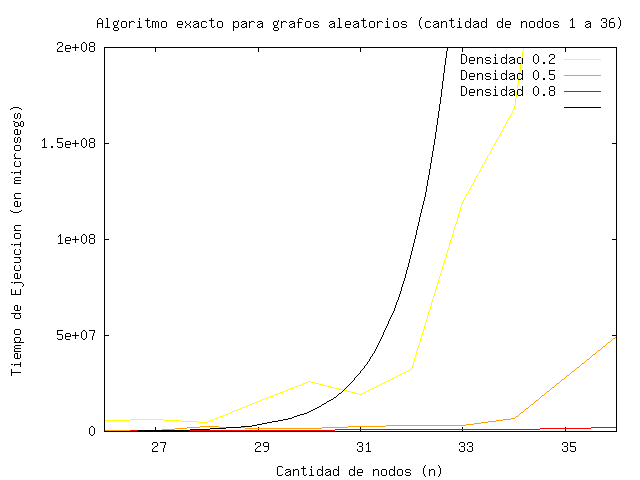
\includegraphics[width=0.8\textwidth]{graficos/tiemposExacto.png}
\begin{center}
Figura 1.1
\end{center}
\end{center}

Como se puede apreciar en el gr\'afico, el tiempo de ejecuci\'on del algoritmo aplicado sobre los distintos grafos seleccionados se comporta de acuerdo a la complejidad te\'orica estimada. Adem\'as, podemos ver que se mantiene muy alejado de la cota para el peor caso ($2^{n}$).

Otro aspecto a tener en cuenta es la notable diferencia de los tiempos en relaci\'on a las diversas densidades. Se puede ver que si la densidad del grafo es baja, el tiempo de busqueda del conjunto independiente de mayor peso es mucho mayor que si se lo busca sobre un grafo de densidad media. Lo mismo sucede entre media y alta densidad. Esto se debe a que al disminuir la cantidad de aristas (menor densidad), la cantidad de conjuntos independientes en el grafo aumenta, ya que mientras menos aristas haya, mayor cantidad de nodos no adyacentes entre si habr\'a. De esta manera, mientras menor sea la densidad, mayor ser\'a la cantidad de conjuntos independientes a tener en cuenta por el algoritmo con el fin de buscar el de mayor peso, por lo que demandar\'a mayor tiempo de ejecuci\'on.

Finalmente estudiaremos la complejidad en funci\'on del tama\~{n}o de la entrada. Sea $t$ el tama\~{n}o de la entrada, $n$ la cantidad de nodos, $m$ la cantidad de aristas ($m_i$ la cantidad de aristas del nodo $i$), $p$ el arreglo de pesos y $a[i]$ las adyacencias del nodo $i$. Tenemos entonces que:

$$t=\log(n)+\sum_{i=1}^{n}\log(p)+\sum_{i=1}^{n}\sum_{j=1}^{m_i}\log(a[i])>\log(n)+\sum_{i=1}^{n}1+\sum_{i=1}^{n}\sum_{j=1}^{m_i}1$$
$$>\log(n)+n+\sum_{i=1}^{n}m>\log(n)+n+nm$$

\hspace{45pt} $\Longrightarrow$ como $T(n) \in O(2^{n})$ y $2^{n}<2^{\log(n)+n+nm}<2^{t} \Longrightarrow T(t) \in O(2^{t})$

\bigskip

\section{Heur\'isticas constructivas}

A continuaci\'on se desarrolar\'a el trabajo realizado sobre heur\'isticas constructivas con el objetivo de reducir significativamente la complejidad temporal a merced de una p\'erdida de eficacia en las soluciones. Para esto, se utilizar\'on distintos algoritmos golosos que tienen en cuenta diversas condiciones sobre los nodos para ir armando una soluci\'on de manera constructiva. Se pensaron varias ideas para buscar aproximarse a la soluci\'on \'optima, todas siguiendo el siguiente esquema de algoritmo goloso:

\begin{verbatim}
mientras haya nodos en el grafo
  maxF = 0 | minF = n
  para cada nodo del grafo
    si grado(nodo) = 0
      agregar nodo a solucion
      borrar nodo del grafo
    sino
      si f(nodo) >= maxF | f(nodo) <= minF
        maxF | minF = f(nodo)
        nodoMax | nodoMin = nodo
  finPara

  agregar nodoMax a solucion
  borrar vecindad de nodoMax
\end{verbatim}

Podemos apreciar que en cada iteraci\'on (del ciclo interno) el algoritmo recorre todos los nodos verificando que se cumpla una condici\'on de acuerdo a una funci\'on aplicada a los mismos (funci\'on $f$). Una vez observados todos los nodos, se agrega el nodo m\'aximo o m\'inimo de acuerdo a la condicion mencionada al conjunto soluci\'on. De inmediato, se procede a borrar la vecindad de dicho nodo del grafo. De esta manera, en cada iteraci\'on, el grafo contendr\'a una cantidad cada vez menor de nodos de modo de garantizar que el algoritmo termina (sale del ciclo principal).

Cabe aclarar que si el grado de los nodos que el algoritmo va recorriendo es igual a 0, inmediatamente son agregados a la soluci\'on. Esto se debe a que, al ser todos los pesos mayores que 0, si un nodo no es adyacente a ning\'un otro (grado 0), siempre deber\'a pertenecer a la soluci\'on.

Las distintas funciones $f$ aplicadas sobre los nodos para armar el conjunto soluci\'on fueron:

\begin{itemize}
\item \textbf{Peso:} en cada iteraci\'on del algoritmo se agrega a la soluci\'on el nodo de mayor peso.
\item \textbf{Grado:} en cada iteraci\'on del algoritmo se agrega a la soluci\'on el nodo de menor grado. La idea de aplicar dicha funci\'on es que, al agregar a la soluci\'on el nodo de menor grado, solo se borrar\'an del grafo los nodos de su vecindad (que es la de menor tama\~{n}o) descartando asi la menor cantidad de nodos posible.
\item \textbf{Peso/Grado:} en cada iteraci\'on del algoritmo se agrega a la soluci\'on el nodo de mayor cociente peso/grado. Simplemente una combinaci\'on de las dos t\'ecnicas mencionadas anteriormente.
\item \textbf{Peso/Vecindad:} en cada iteraci\'on del algoritmo se agrega a la soluci\'on el nodo de mayor cociente peso*grado/pesoVecindad. La intenci\'on en este caso es ponderar tambi\'en el peso y la cantidad de nodos de la vecindad del nodo a agregar a la soluci\'on (si la vecindad del nodo es muy pesada y posee pocos nodos no quiero descartarla).
\end{itemize}

\section*{An\'alisis de eficacia de las heur\'isticas constructivas}

Con el objetivo de decidir que heur\'istica es m\'as eficaz en relaci\'on a la precisi\'on de la soluci\'on obtenida, se realizaron pruebas para 27 grafos distintos generados de manera aleatoria. En los casos que fue posible, se compar\'o el resultado obtenido con la soluci\'on exacta del problema, obtenida por medio del algoritmo exacto presentado anteriormente.

Los grafos generados de manera aleatoria se dividen en 3 tipos seg\'un la cantidad de nodos. Se crearon 9 grafos de cada tipo, con cantidad de nodos 30, 300 y 600. A su vez, cada tipo de grafo se divide seg\'un la densidad del grafo, es decir, de los 9 grafos de cada tipo se crearon 3 con baja, media y alta densidad. El peso de cada uno de los nodos tambi\'en es aleatorio, en un rango de 1 a $n*10$, siendo $n$ la cantidad de nodos. Estos grafos ser\'an utilizados en todas las pruebas que se realizar\'an en el trabajo, tanto para las heur\'isticas constructivas como para las b\'usquedas locales y la metaheur\'istica GRASP.

Para cada uno de los grafos mencionados se ejecutaron todas las heur\'isticas constructivas mencionadas en la secci\'on anterior, obteniendo los siguientes resultados.

\begin{center}
 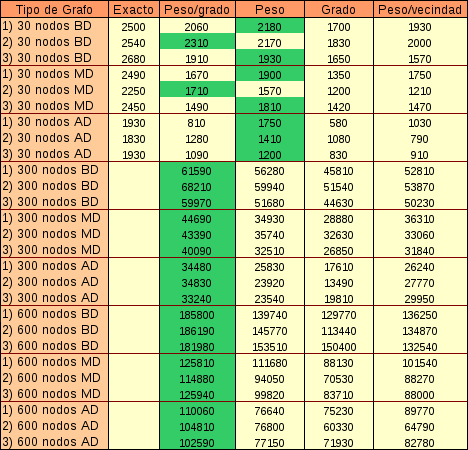
\includegraphics[width=0.75\textwidth]{tablas/tablaHC.png}
\begin{center}
Figura 2.1
\end{center}
\end{center}

Las pruebas realizadas a grafos de 30 nodos pueden ser comparadas con el resultado exacto obtenido por medio del algoritmo de \textit{backtracking}. Como se puede observar, todos los resultados de las heur\'isticas difieren del resultado exacto en distinta medida. Esto es un resultado esperable ya que en la mayor\'ia de los casos todas las heur\'isticas golosas no son eficaces y se pueden encontrar casos en los que el resultado difiera en gran medida del exacto.

En la tabla presentada fueron remarcados los resultados m\'as altos para cada tipo de grafo. Como se puede apreciar, para grafos con 30 nodos, los mejores resultados fueron obtenidos con la heur\'istica de Peso. Sin embargo, para grafos con mayor cantidad de nodos, como los de 300 y 600 nodos, los resultados de la heur\'istica de Peso/grado son ampliamente mejores.

A partir de estos resultados, se puede concluir que la heur\'istica de Peso/Grado es la m\'as eficaz de las heur\'isticas implementadas.  El fundamento m\'as importante para la elecci\'on de la misma fue que los resultados para grafos con gran cantidad de nodos, son mucho m\'as eficaces a las dem\'as heur\'isticas constructivas. Como las heur\'isiticas fueron pensadas para resolver instancias de tama\~{n}o mucho mayor a lo que el algoritmo exacto puede resolver, es razonable que se elija la heur\'istica que mejor se comporte para grafos con gran cantidad de nodos. Adem\'as, para grafos peque\~{n}os los resultados no difieren demasiado de los obtenidos con la heur\'istica de Peso.

En posteriores secciones estudiaremos el comportamiento de la heur\'istica Peso/grado en relaci\'on al tiempo de ejecuci\'on y compararemos dichos resultados con su complejidad te\'orica.

\section*{Complejidad}

El modelo elegido para calcular la complejidad de este algoritmo es el uniforme debido a que lo que la define es la cantidad de nodos y de aristas y como inciden las aristas sobre los nodos. Esto se da porque de ellos depende la cantidad de operaciones que deba realizar el algoritmo de acuerdo a las condiciones de los ciclos.

Antes de analizar las operaciones, cabe aclarar que verificar si dos nodos son adyacentes puede hacerse en tiempo constante, dado que se cuenta con la matriz de adyacencia del grafo. Además se puede obtener el grado asociado a un nodo con la misma complejidad ya que esto se puede realizar viendo el tamaño de su lista de adyacencias.

El cálculo de la complejidad de la heurística es bastante sencilla. Primero observamos el ciclo interno.

\begin{verbatim}
  para cada nodo del grafo //n
    si grado(nodo) = 0  
      agregar nodo a solucion
      borrar nodo del grafo
    sino
      si F(nodo) >= maxF
        maxF = F(nodo)
        nodoMax = nodo
  finPara
\end{verbatim}

En el caso en que el nodo sea de grado $0$, es insertado en la solucion ($O(1)$ al insertar en una lista) y eliminado del grafo ($O(1)$ ya que como el nodo no tiene adyacentes sólo borramos su lista de adyacencias que está vacía).
Es importante comentar que la matriz de adyacencia no es modificada para no aumentar la complejidad, pero que la información que no es modificada no será utilizada ya que está asociada a nodos que fueron borrados.

En el caso en que la relación de peso/grado del nodo obtenido sea mayor o igual al maxF, se actualiza maxF con el número de dicha relación y se lo guarda al nodo en $nodoMax$. En este caso sólo se definen dos variables por lo que es de orden constante. Como dentro del ciclo se realizan sólo operaciones constantes y este recorre todos los nodos del grafo una vez, el orden del ciclo es lineal.

Luego hay dos operaciones:
\begin{verbatim}
  agregar nodoMax a solucion
  borrar vecindad de nodoMax
\end{verbatim}

Agregar $nodoMax$ a la solución es constante debido a que la solución usa como estructura una lista. Para borrar la vecindad de $nodoMax$ del grafo, recorremos las listas de adyacencias y borramos de ellas los nodos que son adyacentes a $nodoMax$. Además, si la lista pertenece a un nodo adyacente a $nodomax$, se borra entera. Como la complejidad de esta operacion se basa en recorrer las listas de adyacencias de todos los nodos, tiene orden $O(n + m)$ ($O(m)$ para los casos en los que no haya nodos aislados).

Por último, el ciclo de afuera se ejecuta mientras haya nodos en el grafo. Teniendo en cuenta que en cada iteracion se elimina por lo menos un nodo del grafo (ya que seguro se borra el nodo que se agrega al grafo) el ciclo se ejecutará como máximo $n$ veces. Esto sumado a que el orden de las operaciones realizadas dentro de él es $O(n + m)$, podemos concluir que la complejidad de la heurística constructiva es $O(n*(n + m))$. Pero como los nodos de grado cero fueron eliminados, sabemos que $n \leq m$, lo que deriva a un orden de $O(n*m)$.

Sin embargo, si se realiza un analisis más minusioso del comportamiento del algoritmo se puede observar lo siguiente. Si el grafo a evaluar resulta muy denso (es decir $m$ cercano $n^2$) la cantidad de nodos de grado alto aumenta proporcionalmente, por lo que la función encargada de borrar la vecindad eliminará del grafo una alta cantidad de nodos en comparación al caso que se trate de un grafo poco denso. Esto último, dará lugar a que la cantidad de veces que itere el ciclo externo disminuya notablemente en grafos densos ya que en cada paso, el grafo resultante contiene una cantidad menor de nodos que en el caso donde la densidad es baja. Este fenómeno de ``equilibro'' podría dar lugar a que el algoritmo en la práctica se comporte mejor de lo que se espera, e incluso que su tiempo de ejecución no dependa de la cantidad de aristas. En la siguiente sección, observaremos empíricamente esta cuestión.

Analizaremos ahora la complejidad en funci\'on del tama\~{n}o de la entrada. Sea $t$ el tama\~{n}o de la entrada, $n$ la cantidad de nodos, $m$ la cantidad de aristas ($m_i$ la cantidad de aristas del nodo $i$), $p$ el arreglo de pesos y $a[i]$ las adyacencias del nodo $i$. Tenemos entonces que:

$$t=\log(n)+\sum_{i=1}^{n}\log(p)+\sum_{i=1}^{n}\sum_{j=1}^{m_i}\log(a[i])>\log(n)+\sum_{i=1}^{n}1+\sum_{i=1}^{n}\sum_{j=1}^{m_i}1$$
$$>\log(n)+n+\sum_{i=1}^{n}m>\log(n)+n+nm$$

\hspace{20pt} $\Longrightarrow$ como $T(n,m) \in O(nm)$ y $nm<\log(n)+n+nm<t \Longrightarrow T(t) \in O(t)$

\section*{An\'alisis de tiempo de ejecución}

Al igual que para el análisis del algoritmo exacto, se generaron grafos aleatorios con 3 tipos de densidades con el fin de evaluar el comportamiento de la heurística constructiva elegida sobre diversos grafos según la cantidad de nodos. Sin embargo, al tratarse de un algoritmo polinomial, la cantidad de nodos analizados será mucho mayor (desde 10 hasta 1400 nodos) con el fin de poder observar con claridad su comportamiento.

Como hemos visto anteriormente, la complejidad de la heurística constructiva resulta del orden $n*m$. Por este motivo, se han incluido en el gráfico las curvas $n^2/25$ y $n^3/15000$ con el fin de observar el comportamiento para grafos de distinta densidad. En principio, los tiempos de ejecución de grafos de alta densidad (donde $m$ tiende a $n^2$) deberían ser similar a la curva $n^3/15000$ mientras que los de baja (donde $m$ tiene a $n$) deberían asimilarse a la curva $n^2/25$.

\begin{center}
 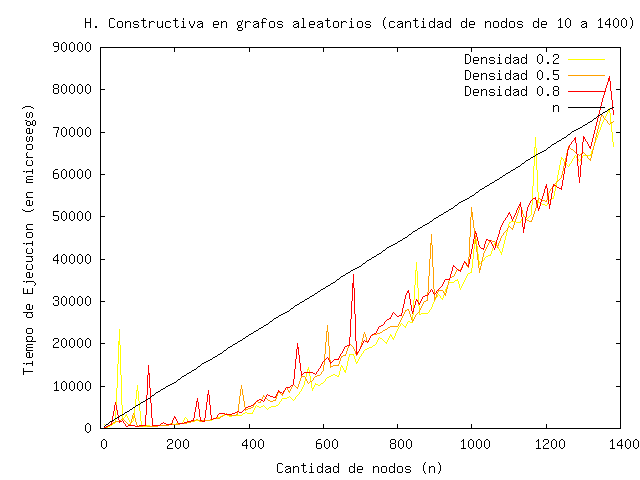
\includegraphics[width=0.7\textwidth]{graficos/tiemposHC.png}
\begin{center}
Figura 2.1
\end{center}
\end{center}

Como se observa, el comportamiento del algoritmo no tiene correspondencia directa con la complejidad teórica calculada, ya que que para grafos de densidad variada, los tiempos de ejecución siempre se comportan de la forma de $n^2$, lo que haría suponer que la complejidad real del algoritmo podría ser de orden cuadrático con respecto a la cantidad de nodos. La razón de esto probablemente radique en el fenómeno de ``equilibro'' mencionado anteriormente en el apartado de complejidad, el cuál logra que, para un grafo promedio, el algoritmo se comporte en un orden de complejidad menor al calculado y dependiendo únicamente de la cantidad de nodos.

\section*{Casos Patol\'ogicos}

En la siguiente secci\'on se estudiar\'a el comportamiento de la heur\'istica constructiva seleccionada anteriormente cuando recibe como par\'ametro un tipo especifico de grafos. Podremos apreciar que en estos casos patol\'ogicos el peso del conjunto independiente m\'aximo retornado difiere notablemente del \'optimo.

Tomemos el siguiente grafo sobre el cual se aplica la heur\'istica:

\begin{center}
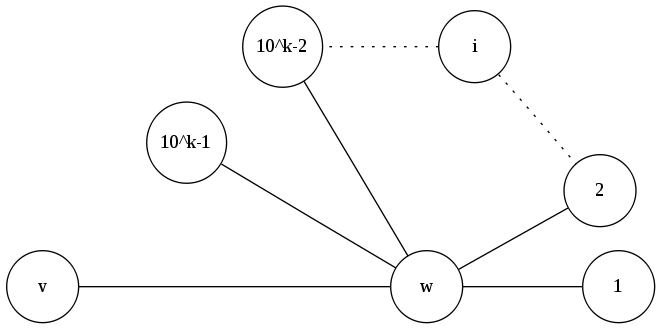
\includegraphics[width=0.7\textwidth]{graficos/casoMaloHC.png}
\begin{center}
Figura 2.1
\end{center}
\end{center}

Supongamos ahora que los nodos numerados desde $1$ a $c^{k}-1$ tienen peso 1, el nodo $v$ peso $c^{k}+1$ y el $w$ $c^{2k}$. De esta manera, como $w$ es adyacente a $c^{k}$ nodos (los nodos numerados y $v$), el cociente $peso(w)/grado(w)=c^{2k}/c^{k}=c^{k}$. Como $v$ es \'unicamente adyacente a $w$, su relacion peso-grado ser\'a $c^{k}+1$. Concluimos entonces que el algoritmo seleccionar\'a a $v$ como primer nodo de la soluci\'on. Al hacer esto, descartamos $w$ como posible nodo perteneciente a la soluci\'on por ser adyacente a $v$. El resto de los nodos (1..$c^{k}-1$) pertenecer\'a a la soluci\'on debido a que no son adyacentes a $v$ ni adyacentes entre ellos. Como el peso de estos \'ultimos nodos mencionados es 1, el peso final de la soluci\'on brindada por la heur\'istica constructiva es $c^{k}+1+\sum_{i=1}^{c^{k}-1}1=c^{k}+1+c^{k}-1=2c^{k}$. A simple vista podemos notar que en realidad, el conjunto independiente de mayor peso es el formado solamente por el nodo $w$ cuyo peso es $c^{2k}$ (tomando $c,k>2$). Finalmente vemos que el peso del conjunto independiente m\'aximo hallado por nuestro algoritmo y el \'optimo difieren en $c^{2k}-2c^{k}=c^{k}(c^{k}-2)$.

Vemos entonces que podemos generar un grafo donde el algoritmo sea tan impreciso como uno desee(ajustando los par\'ametros $c$ y $k$ como se considere necesario).

\bigskip
\section{Heur\'isticas de B\'usqueda Local}

A continuaci\'on se presentar\'an las heur\'isticas de b\'usqueda local implementadas. El objetivo de dichos algoritmos es mejorar una soluc\'on dada (obtenida por medio de alguna de las heur\'isticas constructivas mencionadas), hasta obtener una soluci\'on localmente \'optima. Cada heur\'istica de b\'usqueda local define su concepto de localidad estableciendo una vecindad de soluciones que se revisar\'an para obtener el m\'aximo local. Las b\'usquedas locales implementadas corresponden al siguiente esquema.

\begin{verbatim}
obtengo una solucion (solucionLocal) con una heuristica constructiva 

para i desde 1 hasta cantIteraciones hacer
  pesoMaximoAnterior = peso(solucionLocal)
    solucionLocal = intercambioDeNodo(solucionLocal) o 
                    intercambioDeUnoAMuchos(solucionLocal)
    si peso(solucionLocal) = pesoMaximoAnterior
      devolver solucionLocal

devolver solucionLocal

intercambioDeNodo(solucion)
  diferenciaMaxima = 0
  sacar los nodos de grado 0 de solucion e insertarlos en nodosGradoCero 

  para cada nodo (nodoActual) de solucion
    para cada nodo (adyacenteANodoActual) adyacente a nodoActual
      diferenciaActual = peso(adyacenteANodoActual) - peso(nodoActual)
      si (adyacenteANodoActual no es adyacente a algun nodo de solucion 
         excepto nodoActual y diferenciaActual > diferenciaMaxima)
           diferenciaMaxima = diferenciaActual
           nodoASacar = nodoActual
           nodoAInsertar = adyacenteANodoActual
    finPara
  finPara

  si diferenciaMaxima > 0
    sacar nodoASacar de solucion
    agregar nodoAInsertar en solucion

  insertar todos los nodos de nodosGradoCero en solucion


intercambioDeUnoAMuchos(solucion)
  diferenciaMaxima = 0
  sacar los nodos de grado 0 de solucion e insertarlos en nodosGradoCero

  para cada nodo (nodoActual) de solucion
    nodosAInsertarActual = lista vacia
    para cada nodo (adyacenteANodoActual) adyacente a nodoActual
      si adyacenteANodoActual no es adyacente a algun nodo de solucion excepto nodoActual
        si adyacenteANodoActual no es adyacente a algun nodo de nodosAInsertarActual
          agregar adyacenteANodoActual en nodosAInsertarActual
    finPara
    diferenciaActual = peso(nodosAInsertarActual) - peso(nodoActual)
    si diferenciaActual > diferenciaMaxima
      diferenciaMaxima = diferenciaActual
      nodosAInsertar = nodosAInsertarActual
      nodoASacar = nodoActual
  finPara

  si diferenciaMaxima > 0
    sacar nodoASacar de solucion
    insertar todos los nodos de nodosAInsertar en solucion

  insertar todos los nodos de nodosGradoCero en solucion
\end{verbatim}

Como fue mencionado anteriormente, las b\'usquedas locales implementadas difieren en la forma en que definen su vecindad, pero tienen el mismo esquema b\'asico. Las dos heur\'isticas implementadas obtienen una soluci\'on inicial por medio de alguna de las heur\'isticas constructivas (Peso, Grado, Peso/Grado, Peso/Vecindad) estudiadas en secciones anteriores. Luego, intentan mejorar dicha soluci\'on obtenida una cierta cantidad de veces, establecida mediante el par\'ametro cantIteraciones. Si en alguno de los pasos la soluci\'on no mejorase el algoritmo termina ya que, como los procedimientos utilizados para mejorar la soluci\'on son completamente determin\'isticos, no habr\'ia cambios para las posteriores iteraciones del mismo. Cuando esto sucede, se puede afirmar que la soluci\'on obtenida por la heur\'istica corresponde a un m\'aximo local seg\'un la vecindad definida por dicha heur\'istica.

La primer heur\'istica de b\'usqueda local (a la que llamaremos BL1) mejora la soluci\'on por medio de la funci\'on \textit{intercambioDeNodo}. Esta funci\'on saca un nodo de la soluci\'on que recibe como par\'ametro y agrega otro distinto que forme una soluci\'on v\'alida y que maximice el peso de la soluci\'on. Es decir, saca un nodo de la soluci\'on, al que llamaremos nodoActual y para cada nodo adyacente a nodoActual, verifica si lo puede insertar en la soluci\'on viendo si no es adyacente a ning\'un nodo de la misma. De los nodos adyacentes a nodoActual que se pueden insertar, se elijen s\'olo los de peso mayor al peso de nodoActual ya que son los \'unicos que aumentan el peso total de la soluci\'on. A su vez, se elije el m\'aximo entre dichos nodos para que el peso que se agrega a la soluci\'on sea mayor. Este proceso se repite tomando como nodo nodoActual a todos los nodos de la soluci\'on, por lo que, al terminar de ejecutar la funci\'on se obtendr\'a el nodo a sacar y el nodo a insertar que hacen que el peso de la soluci\'on aumente en m\'axima medida. Es importante aclarar que al sacar un nodo de la soluci\'on s\'olo se pueden agregar los adyacentes a dicho nodo debido a que las soluciones que recibe la b\'usqueda local est\'an generadas por las heur\'isticas constructivas y estas siempre retornan conjuntos independientes maximales. Adem\'as, a partir de lo visto anteriormente, se puede definir la vecindad para esta b\'usqueda local como todas las soluciones que se pueden formar sacando un nodo de la soluci\'on original e insertando otro que forme un conjunto independiente.

La segunda b\'usqueda local implementada (a la que llamaremos BL2) mejora la soluci\'on a trav\'es de la funci\'on \textit{intercambioDeUnoAMuchos}. A diferencia de la b\'usqueda local anterior, esta funci\'on saca un nodo de la soluci\'on y agrega varios nodos nuevos a la misma. M\'as precisamente, saca un nodo de la soluci\'on (nodoActual) y se recorren los nodos adyacentes al mismo (en el orden en que est\'en dispuestos en la lista de adyacencia), agregando en una lista (nodosAInsertarActual) los que no sean adyacentes a alguno de la soluci\'on ni a alguno de dicha lista para asegurar que los nodos de la lista nodosAInsertarActual formen un conjunto independiente. Si la suma de los pesos de la lista mencionada es mayor al peso de nodoActual esta puede ser agregada a la soluci\'on aumentando as\'i su peso. Este paso se repite para cada nodo de la soluci\'on, qued\'andose con la lista de mayor peso que cumpla con las condiciones mencionadas (nodosAInsertar) y con el nodo a sacar (nodoASacar) a partir del cual se la obtuvo. Finalmente, se saca de la soluci\'on el nodo nodoASacar y se agregan a la soluci\'on todos los nodos de la lista nodosAInsertar.

A partir del algoritmo descripto, se puede concluir que la vecindad de la segunda b\'usqueda local se puede definir como todas las soluciones que se pueden armar sacando un nodo y agregando una cierta cantidad de nodos de la manera que fue mencionada anteriormente.

Cabe aclarar que los nodos agregados a cada lista nodosAInsertarActual depende fuertemente del orden en que se encuentren en la lista de adyacencia del nodoActual. Es decir, nodosAInsertarActual puede contener distintos conjuntos independientes, dependiendo del orden en que est\'en los nodos en la lista de adyacencia (en posteriores secciones veremos que ordenar las listas de adyacencias seg\'un el peso de los nodos de mayor a menor ayuda a reducir casos ``patol\'ogicos''). Adem\'as, se puede ver claramente que el conjunto independiente obtenido en dicha lista puede no ser m\'aximo, ya que obtener un conjunto de este tipo ser\'ia una tarea exponencial. Por \'ultimo, es importante mencionar que al comienzo de las funciones \textit{intercambioDeNodo} y \textit{intercambioDeUnoAMuchos} se extraen los nodos de grado 0 (con respecto al grafo original) de la soluci\'on antes de comenzar a mejorar la misma, ya que estos nodos siempre van a formar parte de la soluci\'on \'optima y no tiene sentido sacarlos para intentar insertar sus nodos adyacentes. Al finalizar la mejora de la soluci\'on estos nodos son insertados nuevamente. Como se ver\'a m\'as adelante, realizar esta operaci\'on reduce la complejidad del algoritmo.

\section*{An\'alisis de eficacia}

En la presente sección se intentará observar cuando eficaces resultan las heurísticas de búsqueda local propuestas a la hora de hallar un conjunto independiente de mayor peso. Además, veremos como mejora la calidad de la solución con respecto a cada heurística constructiva presentada anteriormente. El motivo de analizar nuevamente todas las heurísticas es que no necesariamente las soluciones provistas por la mejor heurística hallada harán que las busquedas locales provean los mejores resultados. Es decir, puede ocurrir que, por la forma en la que comporta la busqueda local (en otras palabras, la vecindad a analizar), las soluciones provistas por la heurística golosa de peso/grado no sean las soluciónes iniciales que dén mejores resultados.

Con el fin de realizar las comparaciones mencionadas se optó por realizar una versión extendida de la tabla referida a las heurísticas constructivas. Al igual que antes, cada celda de la tabla contiene el peso de la solución obtenida, aunque para el caso de las búsquedas locales, se muestra también (entre paréntesis) la cantidad de iteraciones realizadas por dicha búsqueda.

\begin{center}
 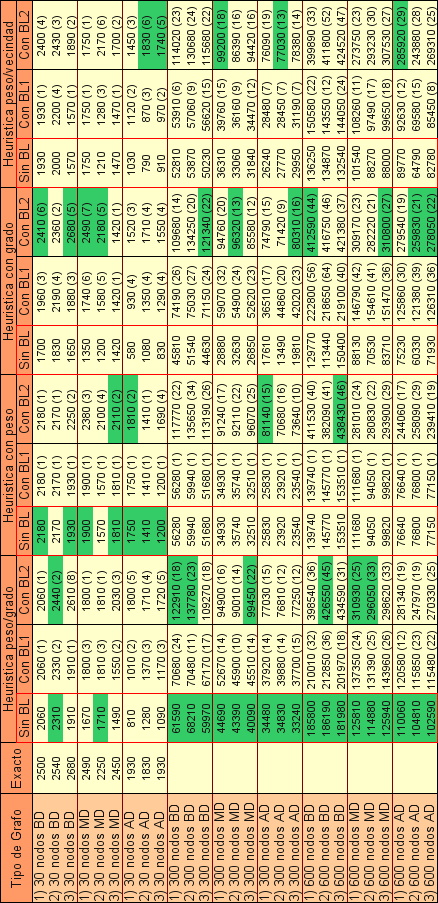
\includegraphics[width=0.75\textwidth]{tablas/tablaHCBL.png}
\end{center}

En primer lugar, podemos observar que la busqueda local 2 resulta \textbf{ámpliamente} superior a la busqueda local 1 para todos los casos evaluados. Lo interesante de esta tabla es ver como se destacan particularmente 2 heurísticas constructivas como generadores de soluciones iniciales ``buenas'' para esta búsqueda. Por un lado la heurística peso/grado muestra ser eficaz tal como lo era por sí sola. Por otra parte, la heurística de grado que resultaba particularmente ineficiente en análisis previos, resulta aún más eficaz que esta en la gran mayoría de los casos.

Otro aspecto interesante a observar es lo que sucede con la cantidad de iteraciones de cada búsqueda en general. La tabla muestra que aún para grafos grandes la cantidad de iteraciones se encuentra acotada por un valor inferior a $100$. Teniendo en cuenta el crecimiento de dicho valor con respecto al tamaño de los grafos y que, debido a cuestiones de complejidad (como veremos más adelante), las grafos sobre los cuales se hará uso este algoritmo no serán mucho más grandes a los grafos analizados (a los sumo del orden de los $10^3$ nodos), podemos concluir que las iteraciones locales nunca superarán un valor del orden de $10^2$. Además, por este motivo y por lo que veremos luego, se puede observar que la cantidad de iteraciones no es un factor determinante sobre el tiempo de ejecución. Por lo tanto, no resulta de importancia al momento de optar por alguna de las 8 busquedas locales (2 por cada heurística constructiva).

Por lo aquí analizado, se puede concluir que la busqueda local 2 junto con la heurística contructiva de grado resultan la combinación más eficaz para la resolución del problema. De aquí en adelante, nos ocuparemos únicamente de dicha heurística.

\section*{Complejidad}

A continuación procederemos a analizar la complejidad de la busqueda local.

\begin{verbatim}
obtengo una solucion (solucionLocal) con la heuristica de grado

para i desde 1 hasta cantIteraciones hacer
  pesoMaximoAnterior = peso(solucionLocal)
    solucionLocal = intercambioDeUnoAMuchos(solucionLocal)
    si peso(solucionLocal) = pesoMaximoAnterior
      devolver solucionLocal

devolver solucionLocal
\end{verbatim}

En primer lugar, se genera una solución inicial con la heuristica de grado elegida. Como vimos anteriormente, dicho algoritmo tiene un costo de orden $O(n*m)$. A continuación, se itera una cantidad constante de veces ya que cantIteraciones es un parámetro acotado, por lo que la complejidad real estará dada por las operaciones definidas dentro del mismo. Es fácil ver que la única operación de complejidad no trivial es la llamada a \textit{intercambioDeUnoAMuchos(solucionLocal)}, ya que el peso del conjunto solución se encuentra almacenado en una variable por lo que su acceso es constante. Por lo tanto, la complejidad estará determinada por esta función cuya primer parte es la siguiente:

\begin{verbatim}
diferenciaMaxima = 0
sacar los nodos de grado 0 de solucion e insertarlos en nodosGradoCero 
\end{verbatim}

Aqui resulta también facil ver que el orden es lineal con respecto a n ya que es necesario recorrer todos los nodos de la solución. La parte interesante del algoritmo es su ciclo principal:

\begin{verbatim}
  para cada nodo (nodoActual) de solucion
    nodosAInsertarActual = lista vacia
    para cada nodo (adyacenteANodoActual) adyacente a nodoActual
      ...
    finPara
    diferenciaActual = peso(nodosAInsertarActual) - peso(nodoActual)
    si diferenciaActual > diferenciaMaxima
      diferenciaMaxima = diferenciaActual
      nodosAInsertar = nodosAInsertarActual
      nodoASacar = nodoActual
  finPara
\end{verbatim}

En primer lugar, el ciclo exterior encargado de recorrer todos los nodos de la solución sería de orden $O(n)$. El ciclo interno recorre los adyacentes a cada uno de esos nodos también en un orden $O(n)$, lo que a primera vista daría a pensar que ambos ciclos en conjunto serían de orden cuadrático. Sin embargo, en total se recorrerán todos los nodos adyecentes a cada nodo de la solución por lo cual como máximo, en caso de que la solución contenga a todos los nodos, se harán $O(m)$ iteraciones (ya que $m \geq n$ porque los nodos aislados ya fueron extraidos previamente de la solución). Por lo tanto, la complejidad de los ciclos anidados es $O(m)$. (Cabe aclarar que el resto de las operaciones no mencionadas resultan trivialmente constantes). Veremos ahora que ocurre con las operaciones dentro del ciclo interno.

\begin{verbatim}
si adyacenteANodoActual no es adyacente a algun nodo de solucion excepto nodoActual
    si adyacenteANodoActual no es adyacente a algun nodo de nodosAInsertarActual
        agregar adyacenteANodoActual en nodosAInsertarActual
\end{verbatim}

La parte importante de este fragmento se encuentra en la verificar que cierto nodo en cuestión (adyacente a un nodo solución) no es adyacente a ningun nodo ya insertado del conjunto de nodos a insertar parcial ni a ningun nodo de la solución. Como verificar una adyacencia requiere tiempo constante, la complejidad estará dada por la cantidad de nodos a verificar. Es fácil ver que esta cantidad está acotada por $n$ ya que los nodos ya insertados son nodos de los adyacentes a los nodos solución por lo cual no pertecen al mismo conjunto que los nodos de la solución. Por este motivo, al tratarse de conjuntos disjuntos de nodos, la suma de dichos elementos debe ser menor a $n$. Por último, como agregar a un conjunto es $O(1)$ entonces es claro que la complejidad de esta parte en cuestión es $O(n)$.

Por lo analizado hasta aquí, podemos concluir entonces que el ciclo general del algorimto es de $O(m*n)$. Por último, resta ver que sucede con el final del pseudocódigo.

\begin{verbatim}
si diferenciaMaxima > 0
    sacar nodoASacar de solucion
    insertar todos los nodos de nodosAInsertar en solucion

insertar todos los nodos de nodosGradoCero en solucion
\end{verbatim}

Como sacar un nodo resulta de orden lineal respecto a $n$ al igual que la última operación, la complejidad total de esta parte es de O(n). Del mismo modo, insertar nuevamente todos los nodos de grado cero también se encuentra acotado por $n$.

Con todo lo analizado, podemos ver que la complejidad total del algoritmo completo es $O(n*m + n + m*n + 2*n) = O(n*m)$.

Finalmente analizaremos la complejidad en funci\'on del tama\~{n}o de la entrada. Sea $t$ el tama\~{n}o de la entrada, $n$ la cantidad de nodos, $m$ la cantidad de aristas ($m_i$ la cantidad de aristas del nodo $i$), $p$ el arreglo de pesos y $a[i]$ las adyacencias del nodo $i$. Tenemos entonces que:

$$t=\log(n)+\sum_{i=1}^{n}\log(p)+\sum_{i=1}^{n}\sum_{j=1}^{m_i}\log(a[i])>\log(n)+\sum_{i=1}^{n}1+\sum_{i=1}^{n}\sum_{j=1}^{m_i}1$$
$$>\log(n)+n+\sum_{i=1}^{n}m>\log(n)+n+nm$$

\hspace{20pt} $\Longrightarrow$ como $T(n,m) \in O(nm)$ y $nm<\log(n)+n+nm<t \Longrightarrow T(t) \in O(t)$

\section*{Casos Patol\'ogicos}

En esta secci\'on se estudiar\'a un caso en el que, dado un tipo de soluci\'on inicial, el algoritmo de busqueda local implementado no realiza una mejora sustancial.

Supongamos que el algoritmo de busqueda local recibe una soluci\'on compuesta por dos nodos que llamaremos $v$ y $w$. Supongamos tambien que el peso de $v$ es 1 y que es adyacente a un \'unico nodo $a$ de peso 2. Adem\'as, $a$ es adyacente a todos los nodos adyacentes a $w$ pero no a este \'ultimo. De esta manera, el algoritmo de busqueda local comenzar\'a por colocar en la lista de nodos a insetrar a $a$, ya que sacando a $v$ de la soluci\'on y agregando a $a$, el peso parcial aumenta en 1. En el siguiente paso, el algoritmo intentara reemplazar $w$ por uno o m\'as nodos adyacentes a el que mejoren la soluci\'on. Como el nodo $a$ es adyacente a todos los adyacentes a $w$, y ya es considerado como uno de los nodos a insertar, no podre agregar ninguno de los nodos adyacentes a $w$ a la lista de nodos a insertar en la soluci\'on. En el caso en que los nodos adyacentes a $w$ tuvieran mucho peso y no fueran adyacentes con el nodo $a$ intercambiado ni entre ellos, no estaria teniendolos en cuenta por lo mencionado anteriormente.

Vemos asi que mientras mayor sea el peso de la vecindad de $w$, mas alejado del mejor intercambio se encontrar\'a la soluci\'on. Este caso patol\'ogico podria ser evitado si en lugar de arrancar los intercambios por el nodo $v$ el algoritmo comenzara por $w$.

\section*{An\'alisis de tiempo de ejecución}

Manteniendo la política utilizada en los ejercicios anteriores, el análisis empiríco se realizó sobre grafos aleatorios. En este caso el algoritmo se corrió para grafos entre 20 y 4000 nodos, nuevamente con 3 tipos de densidades
para poder apreciar si existe una relación entre ellas y el tiempo de ejecución demandado.

Para poder apreciar el comportamiento del algoritmo con respecto a la complejidad teórica se agregaron al gráfico las curvas definidas por $n^3/8000$ y $n^2/9$, dado que como el orden del algoritmo es $n * m$ debe alternar entre esos valores( ya que $n \leq m \leq n^2$).

\begin{center}
 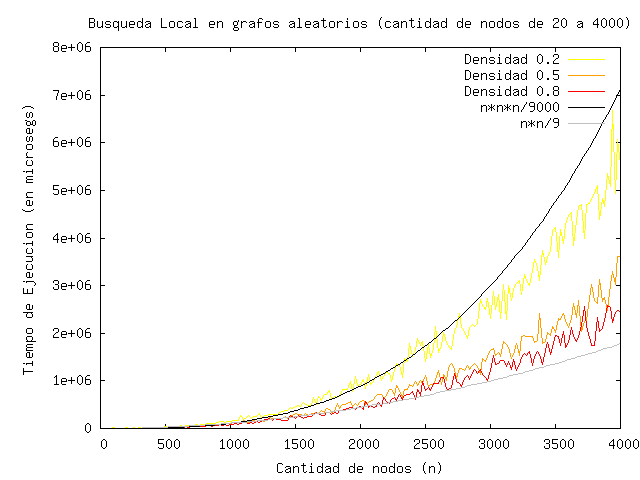
\includegraphics[width=0.7\textwidth]{graficos/tiemposBL.png}
\begin{center}
Figura 4.1
\end{center}
\end{center}

En el gráfico se puede apreciar como la curva de orden $(O(n^3))$ acota superiormente a las curvas que representan los resultados de los tiempos de ejecución para los tres tipos de densidades, mientras la curva de orden $(O(n^2))$ la acota inferiormente lo que coincide con los esperado debido a la relación entre $n$ y $m$. De todas formas se observa que los ejemplos analizados tienden más a una complejidad cuadràtica que cùbica.

Otra característica observable es que la densidad del grafo influye directamente en el tiempo de ejecución del algoritmo, ya que a pesar de no mejorar en complejidad, se puede notar que a medida que se van aumentando las 
densidades disminuye el tiempo requerido. 

\section{Metaheur\'istica GRASP}

La última parte del trabajo es, probablemente, la más interesante. En esta sección se estudiará el comportamiento de la heurística de Grasp, lo que incluye la utilización de las heurísticas anteriores y permite la comparación (para grafos con un número limitado de nodos) de su rendimiento con respecto al valor óptimo obtenido utilizando el algoritmo exacto. Aquí se terminan de tomar las decisiones con respectos a los parámetros a utilizar en las heurísitcas debiendo privilegiar ciertos aspectos por encima de otros. Una vez analizado Grasp, se podrá tener una conclusión en conjunto de lo realizado y detallar los beneficios y las contras de la utilzación de esta heurística para este problema.
A continuación se presenta el pseudocódigo del algoritmo.

\begin{verbatim}
pesoMaximo = 0
para i desde 1 hasta cantIteracionesGrasp
  unaSolucion = heuristicaConstructiva(alfa)
  unaSolucion = busquedaLocal(unaSolucion, cantIteracionesBL)
  si peso(unaSolucion) > pesoMaximo
    laMejorSolucion = unaSolucion
    pesoMaximo = peso(laMejorSolucion)
\end{verbatim}

El algoritmo utilizado consta de un ciclo general que está determinado por la cantidad de iteraciones de Grasp. El ciclo se ejecutará tantas veces como este parámetro lo indique. Para determinar su valor apropiado se efectuarán las pruebas necesarias más adelante. Dentro del ciclo se construye una solución mediante la heurística constructiva, se le aplica búsqueda local y, si consigue mejorar a la óptima obtenida hasta el momento, ocupa su lugar. De esta manera, al terminar el ciclo se obtendrá la mejor solución contrada.

Un punto importante a señalar es el hecho de que las heurísticas constructivas fueron modificadas con el fín de construir distintas soluciones iniciales, tal como indica el esquema de GRASP. Por este motivo, se añadió un parámetro que llamaremos $alfa$ cuyo valor tiene relacion con el factor de aleatoriedad del algoritmo. Más precisamente, en lugar de que la heurística golosa siempre vaya añadiendo a la solución el mejor candidato, agregue alguno de los mejores cantidatos.

Dicho esto, los análisis posteriores se encargarán analizar que valores de los 2 parámetros mencionados son los más adecuados para la metaheurística. 

Por un lado, el alfa determinará qué tan aleatoria será la heurística constructiva. Es importante su buena elección ya que una mala decisión podría limitar notablemente la cantidad de soluciones a verificar, mientras que por otro lado podría construir malas soluciones iniciales lo que influiría negativamente en la eficiencia y eficacia de la búsquela local que se le aplique.

Por otro lado, la otra decisión consiste en determinar una cota para la cantidad de iteraciones de GRASP a realizar. Nuevamente, la relevancia de encontrar un buen valor para éste parámetro se debe a que es necesario encontrar un equilibrio entre la eficiencia temporal y la optimalidad de la solución buscada. Para su determinación resulta fundamental ver qué tanto sigue mejorando la solución a medida que van aumentando las iteraciones para seleccionar el número de iteraciones para el cual la solución deja de conseguir mejoras notables.

\section*{An\'alisis de eficacia}

En la presente secci\'on estudiaremos la eficacia de la metaheur\'istica GRASP en relaci\'on a la precisi\'on de la soluci\'on obtenida. Con este objetivo, compararemos los resultados de GRASP con las mejores heur\'isticas constructivas y de b\'usqueda local seg\'un lo visto en anteriores secciones. Se probar\'a con distintas heur\'isiticas ya que anteriormente se concluy\'o que la mejor heur\'istica constructiva es la de Peso/Grado pero los mejores resultados para la b\'usqueda local se lograron con una heur\'istica constructiva de Grado y la b\'usqueda local 2 (BL2). Es decir, en principio, se desconoce que combinaci\'on de heur\'isticas tendr\'a mejores resultados. 

Las siguientes pruebas realizadas tienen como objetivo estudiar los resultados de la metaheur\'istica variando los par\'ametros de la misma (cantIteracionesGRASP y alfa). Es decir, se intentar\'an decidir los par\'ametros que logren un balance entre la calidad de las soluciones y el tiempo de ejecuci\'on de la metaheur\'istica.

Siguiendo la misma l\'inea utilizada en las pruebas anteriores, para todas las pruebas se utilizaran los grafos aleatorios con densidades baja, media y alta.

\subsection*{An\'alisis de heur\'isticas}

Como se mencion\'o anteriormente, la primer prueba realizada tiene como objetivo decidir que heur\'isiticas constructivas y de b\'usuqeda local hacen los resultados de GRASP sean m\'as eficaces. Para esto se realizar\'an pruebas de GRASP con la mejor heur\'istica constructiva (Peso/Grado) y la heur\'istica constructiva que hace que la b\'usqueda local sea m\'as eficaz (Grado). La b\'usqueda local utilizada fue BL2 ya que se mostr\'o que los resultados son ampliamente mejores que los de BL1.

Las tablas que se presentar\'an a continuaci\'on, muestran la diferencia de los resultados obtenidos de GRASP utilizando la heur\'istica de Grado y los resultados utilizando Peso/Grado (ambas usando BL2 y variando el par\'ametro alfa de 0.1 a 1). Es decir, cada celda de la tabla contiene la diferencia $resultadoGrado - resultadoPeso/Grado$.  Adem\'as, se presentan estos resultados variando la cantidad de iteraciones de GRASP 30, 100 y 300.

\begin{center}
 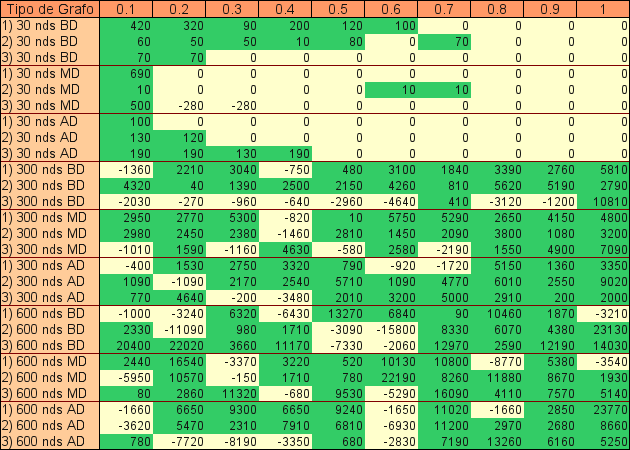
\includegraphics[width=0.75\textwidth]{tablas/tablaGrasp30-1.png}
\begin{center}
Tabla 5.1
\end{center}
\end{center}
\begin{center}
 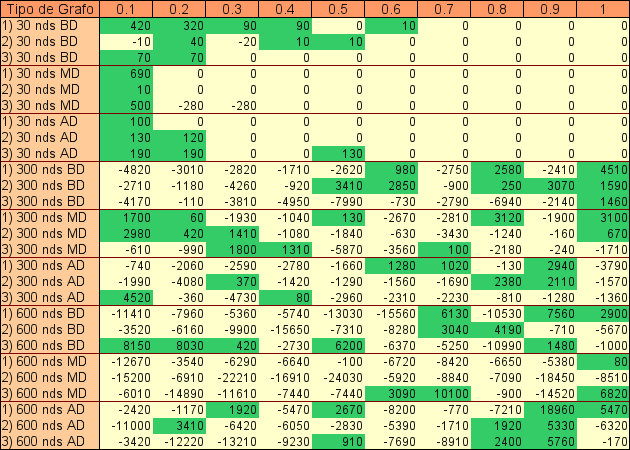
\includegraphics[width=0.75\textwidth]{tablas/tablaGrasp100-1.png}
\begin{center}
Tabla 5.2
\end{center}
\end{center}
\begin{center}
 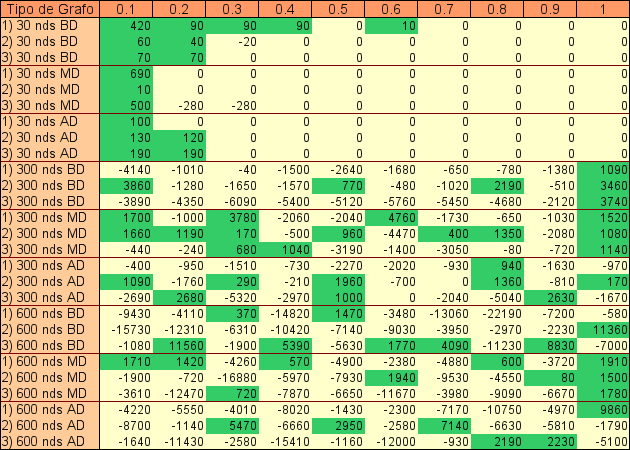
\includegraphics[width=0.75\textwidth]{tablas/tablaGrasp300-1.png}
\begin{center}
Tabla 5.3
\end{center}
\end{center}

Las celdas remarcadas representan los casos en que la diferencia $resultadoGrado - resultadoPeso/Grado$ es mayor que 0, es decir, los casos en los los resultados de GRASP utilizando la heur\'istica de Grado son mayores que utilizando la heur\'istica de Peso/Grado. Como se puede apreciar, cuando la cantidad de iteraciones de GRASP es baja (30) la heur\'istica de Grado es la que otorga los mejores resultados. Sin embargo al aumentar la cantidad de iteraciones la mejores resultados pasan a ser los que se obtienen por medio de la heur\'istica de Peso/Grado. Adem\'as, se puede apreciar que la diferencia en las tablas de 100 y 300 iteraciones es muy remarcada, es decir, los n\'umeros negativos son bastante grandes en m\'odulo, lo que implica que la diferencia entre los resultados es bastante amplia. 

A partir de esto se puede concluir que utilizar la heur\'istica de Grado tiene buenos resultados para poca cantidad de iteraciones, pero al aumentar la cantidad de iteraciones, los resultados se estancan. Por el contrario, si se utiliza la heur\'istica de Peso/Grado, la calidad de los resultados para mayor cantidad de iteraciones aumenta. Esto permite obtener mejores resultados a costa de realizar m\'as cantidad de iteraciones y por tanto, m\'as tiempo de ejecuci\'on. Por esta raz\'on, podemos concluir que utilizar la heur\'istica de Peso/Grado es mejor en cuanto a la calidad de las soluciones, cuesti\'on que resulta de mayor inter\'es que los tiempos de ejecuci\'on del algoritmo.

\section*{Complejidad}

\begin{verbatim}
pesoMaximo = 0
para i desde 1 hasta cantIteracionesGrasp
  unaSolucion = heuristicaConstructiva(alfaRCL)
  unaSolucion = busquedaLocal(unaSolucion, cantIteracionesBL)
  si peso(unaSolucion) > pesoMaximo
    laMejorSolucion = unaSolucion
    pesoMaximo = peso(laMejorSolucion)
\end{verbatim}

En primer lugar, cabe notar que el ciclo principal itera una cantidad constante de veces ya que, tal como se mencionó anteriormente, el parámetro \textit{cantIteracionesGrasp} es un número prefijado que no depende del tamaño de la entrada. Por lo tanto, la complejidad estará dada por el resto de las operaciones dentro del mismo. En particular, la llamada a la heurística contructiva junto con la llamada a la búsqueda local son las operaciones relevantes. Como se mencionó, se optó por utilizar la heurística constructiva peso/grado de complejidad de orden $O(n*m)$. Asímismo, la búsqueda local elegida tiene la misma complejidad, lo que resulta en que la complejidad total de GRASP es de orden $O(n*m)$. A continuación, analizaremos empíricamente este resultado.

A contunuaci\'on analizaremos la complejidad en funci\'on del tama\~{n}o de la entrada. Sea $t$ el tama\~{n}o de la entrada, $n$ la cantidad de nodos, $m$ la cantidad de aristas ($m_i$ la cantidad de aristas del nodo $i$), $p$ el arreglo de pesos y $a[i]$ las adyacencias del nodo $i$. Tenemos entonces que:

$$t=\log(n)+\sum_{i=1}^{n}\log(p)+\sum_{i=1}^{n}\sum_{j=1}^{m_i}\log(a[i])>\log(n)+\sum_{i=1}^{n}1+\sum_{i=1}^{n}\sum_{j=1}^{m_i}1$$
$$>\log(n)+n+\sum_{i=1}^{n}m>\log(n)+n+nm$$

\hspace{20pt} $\Longrightarrow$ como $T(n,m) \in O(nm)$ y $nm<\log(n)+n+nm<t \Longrightarrow T(t) \in O(t)$

\section*{Análisis de tiempo de ejecución}

El siguiente gráfico muestra los tiempos de ejecución del algoritmo de GRASP propuesto. Al igual que antes, se analizan resultados con grafos aleatorios para 3 densidades, en este caso con nodos desde $10$ hasta $800$.

\begin{center}
 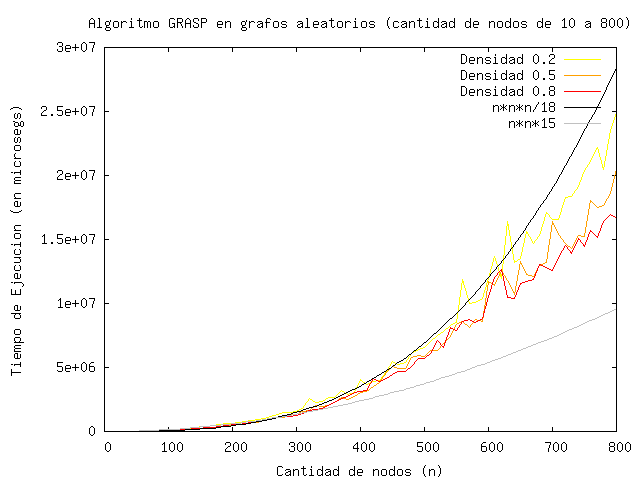
\includegraphics[width=0.75\textwidth]{graficos/tiemposGrasp.png}
\begin{center}
Figura 5.1
\end{center}
\end{center}

Como era de esperarse, el comportamiento del algoritmo es similar al comportamiento de la búsqueda local analizada previamente, ya básicamente el algorimto consiste en realizar sucesivas búsquedas locales. Sin embargo, se puede observar que en este caso la complejidad de GRASP se asemeja más a $n^3$ que en el caso de la búsqueda local. La explicación de este hecho podría recidir en que la búsqueda local de GRASP utiliza la heurística de grado mientras que en GRASP se ha optado por utilizar una búsqueda local con la heurística de peso/grado. De todos modos, se puede observar como claramente el algoritmo respeta la complejidad teórica $O(n*m)$ calculada.

\section{Conclusiones Generales}

\section*{Referencias}
% \begin{itemize}
%  \item Art\'iculo de Wikipedia sobre Programaci\'on Din\'amica
%  \item Art\'iculo de Wikipedia sobre Grafos
%  \item Art\'iculo de Wikipedia sobre Algoritmo de Kruskal
%  \item Art\'iculo de Wikipedia sobre Estructuras Union-Find
%  \item Art\'iculo de Wikipedia sobre Depth/Breadth First Search
% \end{itemize}

\end{document}